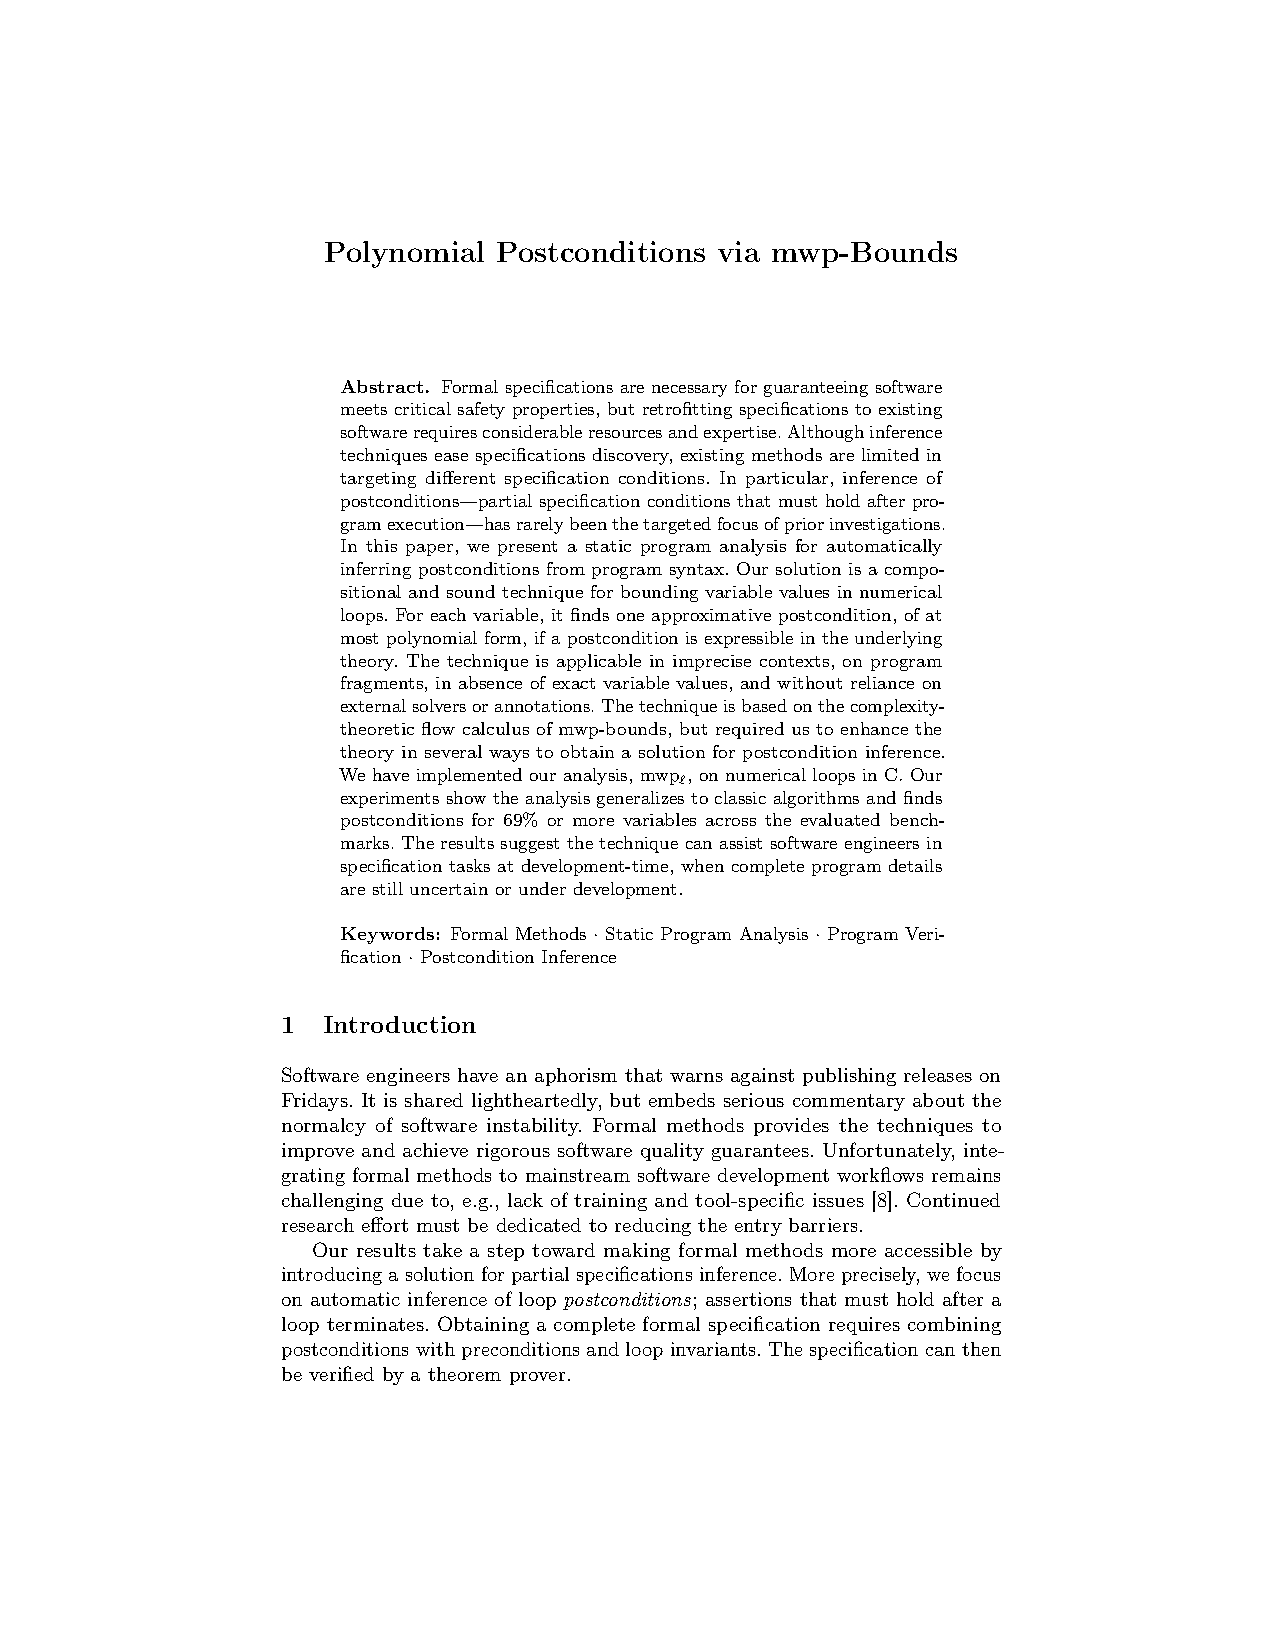
\includepdf[pages={1-},
    addtotoc={
        1,subsection,2,{Introduction},pc-intro,
        2,subsubsection,3,{Problem formulation and solution overview},pc-problem,
        3,subsubsection,3,{Contributions},pc-contrib,
        4,subsection,2,{A High-Level Picture},pc-hl,
        4,subsubsection,3,{Conceptual primer of the flow calculus},pc-primer,
        5,subsubsection,3,{Loop specifications for formal guarantees},pc-specs,
        7,subsection,2,{Technical Preliminaries of the Flow Calculuss},pc-terms,
        7,subsubsection,3,{Imperative language of input programs},pc-lang,
        7,subsubsection,3,{About construction of mwp-matrices},pc-const,
        9,subsubsection,3,{Our starting point of interest: interpreting mwp-matrices},pc-interpret,
        10,subsubsection,3,{Decoding an mwp-matrix by example},pc-decoding,
        11,subsubsection,3,{Interpreting mwp-bounds},pc-bounds,
        11,subsection,2,{Variable-guided matrix exploration},pc-enhancements,
        11,subsubsection,3,{Addressed limitations},pc-limits,
        12,subsubsection,3,{Evaluation for identifying derivable programs},pc-eval,
        14,subsubsection,3,{Variable projection and querying mwp-bounds},pc-projection,
        14,subsubsection,3,{Variable mwp-bounds in presence of failure},pc-bounds-at-failure,
        16,subsection,2,{mwp-bounds as Postconditions},pc-analysis,
        16,subsubsection,3,{Optimal mwp-bounds by form},pc-opt-form,
        17,subsubsection,3,{Variable postcondition search},pc-search,
        18,subsubsection,3,{Program analysis for postcondition inference},pc-prog-analysis,
        18,subsubsection,3,{Postcondition categories as descriptors of variable value behavior},pc-descripts,
        19,subsubsection,3,{Implementing postcondition inference with mwpl},pc-impl,
        20,subsection,2,{Comparison with Related Techniques},pc-comp,
        20,subsubsection,3,{Automatic inference of specification conditions},pc-auto-spec,
        20,subsubsection,3,{A Technical Comparison of Alternative Approaches},pc-alts,
        23,subsection,2,{Experimental Evaluation},pc-expr,
        24,subsubsection,3,{Inference generalizability},pc-gen,
        24,subsubsection,3,{Impact of theoretical enhancements},pc-impact,
        25,subsection,2,{Conclusions and Future Directions},pc-conclusion,
        29,subsection,2,{Appendix A: Application to Program Verification},pc-app-a,
        29,subsection,2,{Appendix B: Technical Details of Analyzer Comparison},pc-app-b,
        32,subsection,2,{Appendix C: Details of Experimental Evaluation},pc-app-c
    }, addtolist={
        2,lstlisting,{Precise context},lst:pc-precise,
        2,lstlisting,{Imprecise context},lst:pc-imprecise,
        5,figure,{Imperative programs and their data flow graphs},fig:prog-dfgs,
        7,figure,{Analysis workflow},fig:analysis-workflow,
        8,figure,{A selection of flow calculus rules},fig:exp-rules,
        10,figure,{DFG of LucidLoop},fig:lucid-dfg,
        13,algorithm,{Evaluation procedure for complex mwp-matrices},alg:mwp-eval,
        15,figure,{The mwp-calculus rules for commands while and loop},fig:loop-rules,
        16,figure,{Improved failure handling},fig:fail-handling,
        21,lstlisting,{LucidLoop},lst:pc-lucidloop,
        21,lstlisting,{Function condition},lst:pc-function,
        21,lstlisting,{Finite iteration},lst:pc-iteration,
        23,table,{Summary of analyzer capabilities},tab:analyzer-comparison,
        24,table,{Experiment results for mwp$_f$ and mwp$_\ell$ with totals and (mean)},tab:pc-results,
        29,lstlisting,{LucidLoop verified in Dafny},list:pc-dafny,
        31,figure,{Postcondition analysis scopes.},fig:pc-scoping,
        31,lstlisting,{mwp: example 3.4},lst:pc-ex34,
        31,lstlisting,{mwp: not infinite \#4},lst:pc-notinfty4,
        31,lstlisting,{Linear: \#02},lst:linear2,
        32,table,{Summarized benchmark suite characteristics},tab:pc-bench-summary},
    pagecommand={\thispagestyle{empty}%
    \addtoindexm{DIG}{20}
    \addtoindexm{Dafny}{29}
    \addtoindexm{Daikon}{20,22,23,30,31}
    \addtoindexm{EvoSpex}{20}
    \addtoindexm{KoAT}{20,21,23,30,31,32}
    \addtoindexm{Duet}{2,20,21,22,23,30,31}
    \addtoindexm{Hoare triple}{6}
    \addtoindexm{abstract interpretation}{20}
    \addtoindexm{choice vector}{12,13,14,15,17}
    \addtoindexm{dynamic program analysis}{20,22}
    \addtoindexm{honest polynomial}{11}
    \addtoindexm{imperative programs}{2,4,5,7,18,19}
    \addtoindexm{invariant}{1,2,6,20,21,22,23,29,30,31}
    \addtoindexm{mwp-matrix}{7,8,9,10,11,12,13,14,15,16,17,18}
    \addtoindexm{monomial}{9,13,14,17}
    \addtoindexm{mwp-bound}{3,4,5,11,12,14,15,16,17,18,19,22,24,25}
    \addtoindexm{nondeterminism}{5,8,9,11}
    \addtoindexm{precondition}{2,6,20,29,32}
    \addtoindexm{program trace}{20,22,23,30}
    \addtoindexm{pymwp}{3,13,19,23,30,32}
    \addtoindexm{quasi-invariant}{18}
    \addtoindexm{specifications}{1,2,5,6,20,21,22,25}
    \addtoindexm{state explosion}{11}
%    \addtosymbols{cv}{10}
%    \addtosymbols{cv}{13}
%    \addtosymbols{cv}{9}
%    \addtosymbols{hoare}{4}
%    \addtosymbols{hp}{8}
%    \addtosymbols{infty}{10}
%    \addtosymbols{infty}{11}
%    \addtosymbols{infty}{12}
%    \addtosymbols{infty}{13}
%    \addtosymbols{infty}{17}
%    \addtosymbols{infty}{18}
%    \addtosymbols{infty}{5}
%    \addtosymbols{infty}{6}
%    \addtosymbols{infty}{7}
%    \addtosymbols{infty}{8}
%    \addtosymbols{infty}{9}
%    \addtosymbols{k}{10}
%    \addtosymbols{k}{13}
%    \addtosymbols{k}{7}
%    \addtosymbols{k}{8}
%    \addtosymbols{k}{9}
%    \addtosymbols{mwpi}{6}
%    \addtosymbols{mwpi}{7}
%    \addtosymbols{m}{5}
%    \addtosymbols{m}{6}
%    \addtosymbols{m}{7}
%    \addtosymbols{m}{8}
%    \addtosymbols{m}{11}
%    \addtosymbols{m}{12}
%    \addtosymbols{m}{17}
%    \addtosymbols{lnot}{4}
%    \addtosymbols{post}{4}
%    \addtosymbols{pre}{4}
%    \addtosymbols{p}{5}
%    \addtosymbols{p}{6}
%    \addtosymbols{p}{7}
%    \addtosymbols{p}{8}
%    \addtosymbols{p}{11}
%    \addtosymbols{p}{12}
%    \addtosymbols{p}{17}
%    \addtosymbols{ttrue}{4}
%    \addtosymbols{vlist}{8}
%    \addtosymbols{w}{5}
%    \addtosymbols{w}{6}
%    \addtosymbols{w}{7}
%    \addtosymbols{w}{8}
%    \addtosymbols{w}{11}
%    \addtosymbols{w}{12}
%    \addtosymbols{w}{17}
%    \addtosymbols{vdash}{4}
%    \addtosymbols{xprime2}{5}
%    \addtosymbols{zero}{5}
%    \addtosymbols{zero}{6}
%    \addtosymbols{zero}{7}
%    \addtosymbols{zero}{8}
%    \addtosymbols{zero}{11}
%    \addtosymbols{zero}{12}
    }]{pdf/pubs_pc.2025.pdf}